\documentclass[11pt]{article}

\usepackage[utf8]{inputenc}
\usepackage[T1]{fontenc}
\usepackage{amsmath, amssymb, amsthm}
\usepackage{graphicx}
\usepackage{geometry}
\usepackage{doi}
\usepackage{hyperref}
\hypersetup{colorlinks=true, linkcolor=blue, citecolor=blue, urlcolor=blue}

\geometry{a4paper, margin=2.5cm}

\graphicspath{{../code/}{./}}

\newtheorem{proposition}{Proposition}
\newtheorem{definition}{Definition}
\newtheorem{remark}{Remark}

\newcommand{\Heis}{\mathrm{Heis}_3(\mathbb{Z}/q\mathbb{Z})}
\newcommand{\DPi}{\Delta_\Pi}
\newcommand{\fQ}{f_Q}
\newcommand{\Lap}{L_\Pi}

\title{\textbf{Quantum Fisher Information as a Spectral Entanglement Witness:\\
the Projective Stability Gap and the Origin of Scale-Free Growth}}
\author{J\'er\^ome Beau\\
\small Independent Researcher, France\\
\small \texttt{jerome.beau@cosmochrony.org}}
\date{\today}

\begin{document}

\maketitle

\begin{abstract}
A recent inelastic-neutron-scattering experiment on the heavy-fermion strange metal
$\mathrm{Ce}_3\mathrm{Pd}_{20}\mathrm{Si}_6$ reports a scale-free increase of the quantum Fisher information (QFI)
density as the strange-metal state forms, witnessing high multipartite entanglement~\cite{Mazza2026}.
We ask whether this signature is reproduced by the non-injective projection framework of Cosmochrony, and we
isolate the structural condition under which it is.
We first reduce the QFI density to the projective spectral data:
using linear response, the QFI density is a weighted integral of the imaginary part of the dynamical
susceptibility, whose infrared behaviour is controlled by the projective stability gap $\DPi$ and the edge
spectral weight of the projective stability operator $\Lap$.
This yields a clean dichotomy.
A finite gap forces the QFI density to saturate; a gap that closes with an anomalous edge density of states of
exponent $a$ forces $\fQ(T)\sim T^{1-a}$, so that scale-free growth requires $a>1$.
We then evaluate the two ingredients by exact diagonalisation.
The single winding sector $w=2$ reduces to the critical almost-Mathieu (Harper) operator at flux $2/q$;
its gap closes as $\DPi\sim q^{-1}$ but its edge spectral dimension is $d_s\to 2$, giving $a\to 1$, the marginal
boundary, hence only logarithmic growth.
The full Cayley substrate of $\Heis$, whose homogeneous growth dimension is $D=4$, instead has an edge spectral
dimension $d_s\approx 4$, giving $a\approx 2$ and $\fQ(T)\sim T^{-1}$, a genuine power law.
The conclusion is structural: in this framework the scale-free QFI growth is a property of the full nilpotent
substrate and not of any isolated composite, consistent with the collective, multipartite character of the
measured entanglement.
The required thermal closure $\DPi(T)\sim T$ is obtained at the level of the effective heat-kernel response: the
framework identifies the diffusion scale with inverse temperature, and the induced linear-response flow gives
$\DPi(T)=\tfrac{d_s}{2}T$, so that the chain from the nilpotent substrate to the linear prediction
$\fQ(T)\sim T^{-1}$ closes within the effective response regime.
The predicted exponent is of the right order but steeper than observed.
Numerically, the Born--Infeld bounded-response correction can soften the effective exponent from the linear value
$\alpha_{\mathrm{th}}=1$ towards the observed $\alpha_{\mathrm{exp}}\approx 0.7$, with a size-stable crossing at a
partial substrate saturation.
The asymptotic exponent and the saturation level realised by the material remain open.
\end{abstract}

\noindent\textbf{Keywords:} quantum Fisher information; multipartite entanglement; strange metals; non-injective
projection; spectral stability gap; almost-Mathieu operator; spectral dimension; Cosmochrony.

\newpage
\tableofcontents

\newpage
\section{Introduction}
\label{sec:intro}

The quantum Fisher information (QFI) provides a measurable, model-independent lower bound on multipartite
entanglement.
For a thermal state and a collective witness operator $\hat O$, the QFI density is obtained from the imaginary
part of the dynamical susceptibility through the relation~\cite{Hauke2016}
\begin{equation}
\fQ(T) = \frac{4}{\pi}\int_0^\infty d\omega \, \tanh\!\Big(\frac{\omega}{2T}\Big)\,\chi''(\omega,T),
\label{eq:qfi}
\end{equation}
so that an entanglement statement is converted into a spectral statement about the response function.
A recent experiment on the Kondo-destruction strange metal $\mathrm{Ce}_3\mathrm{Pd}_{20}\mathrm{Si}_6$ reports
that the spin QFI density increases without a characteristic scale as the strange-metal state forms with
decreasing temperature, reaching a value that bounds the entanglement depth below by nine~\cite{Mazza2026}.
The scale-free character is the entanglement-side signature of local quantum criticality, in which the
low-energy dynamics acquires an $\omega/T$ scaling form~\cite{Si2001}.

This note asks whether the non-injective projection framework of Cosmochrony~\cite{Cosmochrony} reproduces this
signature, and, more usefully, isolates the exact structural condition that controls it.
The framework already contains two entanglement witnesses, neither of which is the QFI: the projection entropy
$S_\Pi$, which bounds the strength of Bell--CHSH violations~\cite{Beau2026b}, and an effective entanglement
observable $E_{\mathrm{eff}}(C)=\DPi(C)\,(1-C^\nu)$ associated with discrete spectral reorganisation
events~\cite{Cosmochrony}.
Both are built from the projective stability gap $\DPi$, which is defined as the lowest positive eigenvalue of the
projective stability operator $\Lap$ restricted to the winding sector $w=2$~\cite{Cosmochrony, Beau2026g}.
This common dependence on $\DPi$ is the hook used below: equation~\eqref{eq:qfi} also depends on the substrate only
through the spectrum of $\Lap$.

The plan is as follows.
Section~\ref{sec:reduction} carries out the reduction of the QFI density to the projective spectral data and
states the resulting dichotomy.
Section~\ref{sec:w2} evaluates the single winding sector $w=2$, which reduces to a critical almost-Mathieu
operator and is found to be marginal.
Section~\ref{sec:full} evaluates the full substrate, which is found to give power-law growth.
Section~\ref{sec:discussion} compares with the experiment, contrasts the QFI with the effective entanglement
observable, and lists the open directions.
Every quantitative claim is labelled as structural (derived from the framework), numerical (established by exact
computation), conditional (subject to a stated input), or open.

\section{Reduction of the QFI density to the projective spectral data}
\label{sec:reduction}

\subsection{Dynamical susceptibility from the stability operator}

In the linear-response regime the dissipative response of a collective witness operator coupled to the substrate is
the imaginary part of the retarded Green operator built on $\Lap$.
In the spin channel of a metal the relevant dynamics is relaxational, so a mode of eigenvalue $\lambda$ contributes
a Debye susceptibility, and the full response is the spectral average
\begin{equation}
\chi''(\omega,T) = \int_{\DPi}^{\Lambda} d\lambda \; W(\lambda)\,\frac{\omega\,\lambda}{\omega^2+\lambda^2},
\label{eq:chi}
\end{equation}
where $W(\lambda)=\rho(\lambda)\,w(\lambda)$ is the effective spectral weight, $\rho(\lambda)$ is the density of
states of $\Lap$, $w(\lambda)$ is the matrix-element weight of the witness operator, and $\Lambda$ is an
ultraviolet band cutoff.
The lower limit $\DPi$ is the projective stability gap: it is the infrared scale that cuts off the response.
This is the structural role of $\DPi$ in the present context.
\emph{Status: structural.}
The relaxational form and a flat weight $w(\lambda)\equiv 1$ are working assumptions, recorded as inputs in
Section~\ref{sec:discussion}.

\begin{remark}[Status of the relaxational response]
The word ``relaxational" is used here in the standard linear-response sense of a Debye-type dissipative
susceptibility in the spin channel.
It does not mean that the relational substrate carries a fundamental time dynamics.
In the axiomatic formulation of the framework the primitive structure is the admissible non-injective projection,
and observable ordering is induced by admissibility.
Accordingly, $e^{-t\Lap}$ is used below as an effective heat-kernel response flow, not as a microscopic evolution
law for the substrate.
\end{remark}

\subsection{Gapped branch: saturation}

If $\DPi>0$ stays finite as $T\to 0$, then $\chi''(\omega)\simeq\kappa\,\omega$ at low frequency with
$\kappa=\int W(\lambda)/\lambda\,d\lambda<\infty$, the integral being finite precisely because of the gap.
Equation~\eqref{eq:qfi} then gives
\begin{equation}
\fQ(T)\;\xrightarrow{T\to 0}\;\frac{4}{\pi}\int_0^\infty \chi''(\omega)\,d\omega = \mathrm{const},
\end{equation}
since $\tanh(\omega/2T)\to 1$ and the integral converges.
The QFI density saturates and the entanglement depth is bounded.
\emph{Status: structural.}

\subsection{Critical branch: scale-free growth}

If instead the gap closes and the response admits a local-critical scaling window
$\chi''(\omega,T)=T^{-a}\,\Phi(\omega/T)$, then two asymptotic regimes must be distinguished.
The oddness of $\chi''$ and regularity at fixed nonzero temperature require $\Phi(x)\sim x$ as $x\to 0$, whereas the
zero-temperature edge exponent is encoded in the large-argument regime $\Phi(x)\sim x^{a}$ over the scaling window
before the ultraviolet cutoff.
Substituting $x=\omega/T$ in equation~\eqref{eq:qfi} gives the temperature-dependent scaling contribution
\begin{equation}
\fQ(T)\;\sim\;T^{1-a}\int_0^{\Lambda/T} dx\,\tanh(x/2)\,\Phi(x),
\label{eq:scaling}
\end{equation}
whose proportionality constant is cutoff-dependent but whose power of $T$ is fixed by the scaling window.
Scale-free growth as $T\to 0$ therefore requires $a>1$; the marginal case $a=1$ produces logarithmic growth, and
$a<1$ does not grow.
At zero temperature the same edge exponent reads $\chi''(\omega)\sim\omega^{a}$ within the scaling window, which by
equation~\eqref{eq:chi} is controlled by an edge spectral weight $W(\lambda)\sim\lambda^{a-1}$.
Equivalently, writing the integrated counting function as $N(\lambda)\sim\lambda^{p}$ near $\lambda\to 0^+$, a flat
matrix-element weight gives $p=a$ and a spectral dimension $d_s=2p=2a$.
\emph{Status: structural, conditional on the scaling form and on the stated ultraviolet cutoff.}

\subsection{The dichotomy}

The reduction shows that the experimentally observed behaviour is equivalent to two well-posed spectral statements
about $\Lap$:
\begin{enumerate}
\item the gap closes (otherwise the gapped branch forces saturation);
\item the edge density of states is anomalous with exponent $a>1$ (otherwise the growth is at most marginal).
\end{enumerate}
Both are computable on the Cayley graphs of $\Heis$ used as relaxation graphs in the spectral admissibility
sub-programme~\cite{Beau2026a13, Beau2026a1note}.
The remaining two sections evaluate them, first in a single winding sector and then on the full substrate.

\section{The single winding sector \texorpdfstring{$w=2$}{w=2}}
\label{sec:w2}

\subsection{Reduction to the critical almost-Mathieu operator}

The relaxation graph is the Cayley graph of $\Heis$ with the symmetric generating set $\{X^{\pm 1}, Y^{\pm 1}\}$,
a connected $4$-regular graph of order $q^3$~\cite{Beau2026a13}.
The winding sector is the Weil block of central character $c$ in the decomposition
$\rho_{\mathrm{aff}}=\rho_0\oplus\bigoplus_{c=1}^{q-1}\rho_c$.
In the block of character $c$ the generators $X,Y$ act as the shift and clock operators, and the adjacency reduces
to the Harper operator at flux $\alpha=c/q$,
\begin{equation}
\big(A^{(c)}f\big)(j) = f(j-1)+f(j+1)+2\cos\!\Big(\frac{2\pi c\,j}{q}\Big)f(j), \qquad j\in\mathbb{Z}/q\mathbb{Z},
\label{eq:harper}
\end{equation}
with normalised Laplacian $L^{(c)}=I-A^{(c)}/4$.
The isotropic coupling places equation~\eqref{eq:harper} exactly at the self-dual critical point of the
almost-Mathieu family~\cite{Hofstadter1976}.
The sector $w=2$ is the block $c=2$, and $\DPi|_{w=2}=\lambda_{\min}^{+}(L^{(2)})$.
\emph{Status: structural (identification of the sector with the Weil block).}

\subsection{Numerical result}

Exact diagonalisation of $L^{(2)}$ for all primes $5\le q\le 1009$, with a control run to $q=2003$, gives the
following.
The gap closes as $\DPi(q)\sim q^{-\beta}$ with $\beta\to 0.999$, that is $\DPi\sim 1/q$, the Landau-level spacing
of the small-flux Harper edge.
The integrated edge counting function obeys $N(\lambda)\sim\lambda^{p}$ with $p\to 1$ as $q\to\infty$, so the edge
spectral dimension is $d_s\to 2$ and the susceptibility exponent is $a\to 1$.
By equation~\eqref{eq:scaling} this is the marginal case: the single winding sector predicts only logarithmic
growth, $\fQ\sim\log(1/T)$, not a power law.
Figure~\ref{fig:w2} shows the gap closure and the edge counting function.
\emph{Status: numerical (exact diagonalisation, clean convergence).}

\begin{figure}[t]
\centering
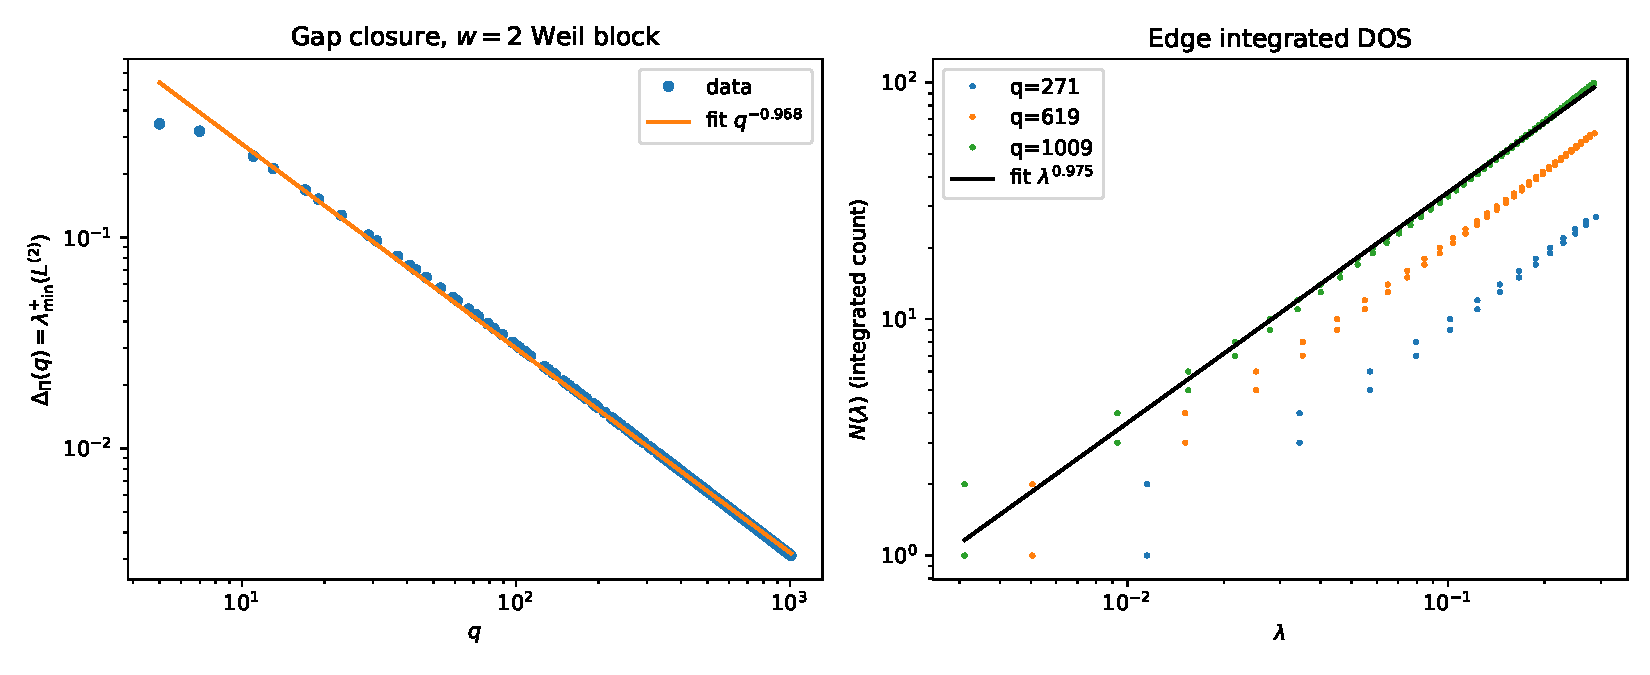
\includegraphics[width=0.92\textwidth]{qfi_edge_dos}
\caption{Single winding sector $w=2$ (critical almost-Mathieu operator at flux $2/q$).
Left: closure of the projective stability gap, $\DPi(q)\sim q^{-1}$.
Right: integrated edge density of states $N(\lambda)$ for representative primes, with the fitted exponent
$p\to 1$, hence $d_s\to 2$ and $a\to 1$ (marginal).}
\label{fig:w2}
\end{figure}

The physical reading is that near its band edge the small-flux Harper operator is a Landau-level problem, a
one-dimensional chain dressed by an effective magnetic flux, so the edge density of states is constant
($d_s=2$) and the level spacing scales as the flux ($\DPi\sim 1/q$).
The sector $w=2$ therefore sits exactly on the marginal boundary $a=1$: the gap closes, but the edge weight is too
weak, by exactly the marginal amount, to produce power-law growth.

\section{The full substrate}
\label{sec:full}

\subsection{Numerical result}

The full normalised Laplacian $L=I-A/4$ of the Cayley graph of $\Heis$, of order $q^3$, was evaluated first by
dense diagonalisation for $q\le 19$.
The global gap closes as $\lambda_2(q)\sim q^{-2}$, set by the lowest abelian (torus) mode of the abelianisation
$(\mathbb{Z}/q\mathbb{Z})^2$.
The edge density of states, however, is not governed by this abelian bottom.
On the window $\lambda\in[0.05,0.20]$ above the lowest mode, the integrated counting function obeys
$N(\lambda)\sim\lambda^{p}$, with $p\approx 2.15$ at $q=19$.
The exact block decomposition of Section~\ref{sec:stacking} lets the full spectrum be assembled at cost $O(q^4)$,
rather than by diagonalising a $q^3\times q^3$ matrix, reaching $q=151$.
The exponent then extrapolates in $1/q$ to $p_\infty\approx 1.96$, hence $d_s\to 4$ and $a\to 2$, the homogeneous
growth dimension $D=4$ of $\Heis$ (Bass--Guivarc'h); the same procedure gives $p_\infty\approx 0.98$ for the single
$w=2$ block, hence $d_s\to 2$ and $a\to 1$.
A sliding log-log slope of $N(\lambda)$ for the full substrate remains at or above $2$ across the edge and never
approaches $1$, so the abelian two-dimensional regime exists only at the lowest mode and does not control the
density of states.
Figure~\ref{fig:full} shows the global gap, the edge counting function, and the sliding spectral dimension up to
$q=23$; Figure~\ref{fig:refine} shows the $q$-convergence and the band-stacking mechanism.
\emph{Status: numerical (exact, by block assembly to $q=151$): the full substrate has $a\to 2$ and the single
$w=2$ block $a\to 1$.}

\begin{figure}[t]
\centering
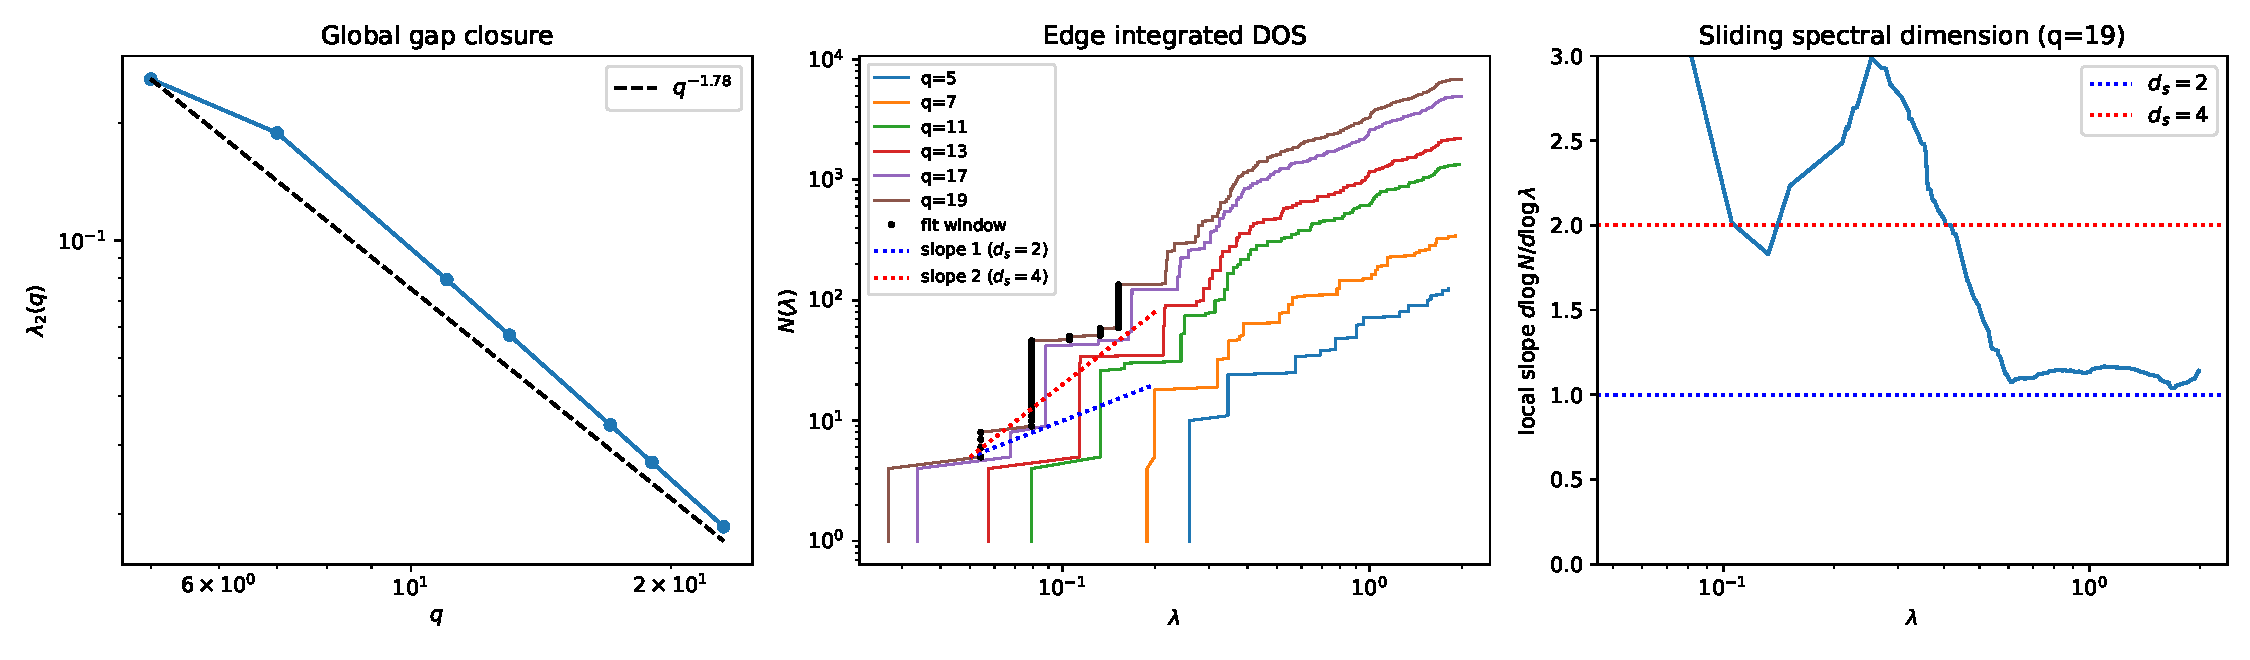
\includegraphics[width=0.99\textwidth]{heis_full_edge_dos}
\caption{Full Cayley substrate of $\Heis$.
Left: global gap closure $\lambda_2(q)\sim q^{-2}$, set by the abelian torus mode.
Centre: edge integrated density of states against reference slopes $1$ ($d_s=2$) and $2$ ($d_s=4$); the data
follow slope $2$.
Right: sliding local slope, remaining at or above $2$ across the edge, hence $d_s\approx 4$, $a\approx 2$.}
\label{fig:full}
\end{figure}

\subsection{Consequence}

By equation~\eqref{eq:scaling} the value $a\approx 2$ gives $\fQ(T)\sim T^{-(a-1)}\approx T^{-1}$, a genuine
power law.
The contrast with Section~\ref{sec:w2} is the central result.
\begin{proposition}[Origin of scale-free growth]
\label{prop:origin}
In this framework the scale-free growth of the quantum Fisher information density is a property of the full
nilpotent substrate, of homogeneous dimension $D=4$, and not of any isolated winding sector.
A single composite $w=2$ is marginal ($a=1$, logarithmic), whereas the full substrate is power-law
($a\approx 2$).
\end{proposition}
\noindent This is consistent with the measured entanglement being multipartite, of depth at least nine: a
collective entanglement over many fibres cannot be carried by a single winding, and the computation confirms this
quantitatively.

\begin{remark}[Complementarity with the superconducting role of $w=2$]
The marginality of the single $w=2$ sector found here is not in tension with the central role of $w=2$ in the
superconductivity construction~\cite{Beau2026g}, where the stabilisation and condensation of the $w=2$ composite is
the pairing mechanism.
The two regimes are complementary rather than contradictory: a condensed $w=2$ composite carries superconductivity,
whereas the full, fluctuating and uncondensed substrate carries the scale-free multipartite entanglement of the
strange metal.
This complementarity is the structural reason the superconductivity analysis and the present one are kept as separate
notes.
\end{remark}

\subsection{Mechanism: band stacking}
\label{sec:stacking}

The contrast between the single sector and the full substrate has an exact structural origin.

\begin{proposition}[Exact block decomposition]
\label{prop:decomp}
The spectrum of the full normalised Laplacian of the Cayley graph of $\Heis$ is, with multiplicity,
\begin{equation}
\mathrm{spec}(L) =
\underbrace{\Big\{\,1-\tfrac14\big(2\cos\tfrac{2\pi k_1}{q}+2\cos\tfrac{2\pi k_2}{q}\big)\,\Big\}_{
(k_1,k_2)\in(\mathbb{Z}/q\mathbb{Z})^2}}_{\text{abelian torus, } q^2 \text{ modes}}
\;\cup\; \bigcup_{c=1}^{q-1}\;\mathrm{spec}\big(L^{(c)}\big)\ \text{(multiplicity } q),
\label{eq:decomp}
\end{equation}
where $L^{(c)}=I-A^{(c)}/4$ is the Harper Laplacian of equation~\eqref{eq:harper} at flux $c/q$.
The identity holds to machine precision.
\end{proposition}

The full edge density of states is therefore the stack of one abelian torus band, of spectral dimension $d_s=2$,
and $q-1$ Harper bands, each itself $d_s=2$ near its own edge but gapped at a staggered scale $\Delta(c)$ that
increases with the flux $c/q$.
Stacking $\sim q$ two-dimensional band edges at staggered thresholds reconstructs a four-dimensional edge density
of states, $d_s=4$.
This is the structural reason why the scale-free growth is a property of the full substrate and not of any single
winding sector, as stated in Proposition~\ref{prop:origin}: a single band edge is two-dimensional and marginal,
whereas their staggered stack is four-dimensional and power-law.
\emph{Status: structural (the decomposition~\eqref{eq:decomp}), numerical (the staggering and the reconstructed
$d_s=4$).}

\begin{figure}[t]
\centering
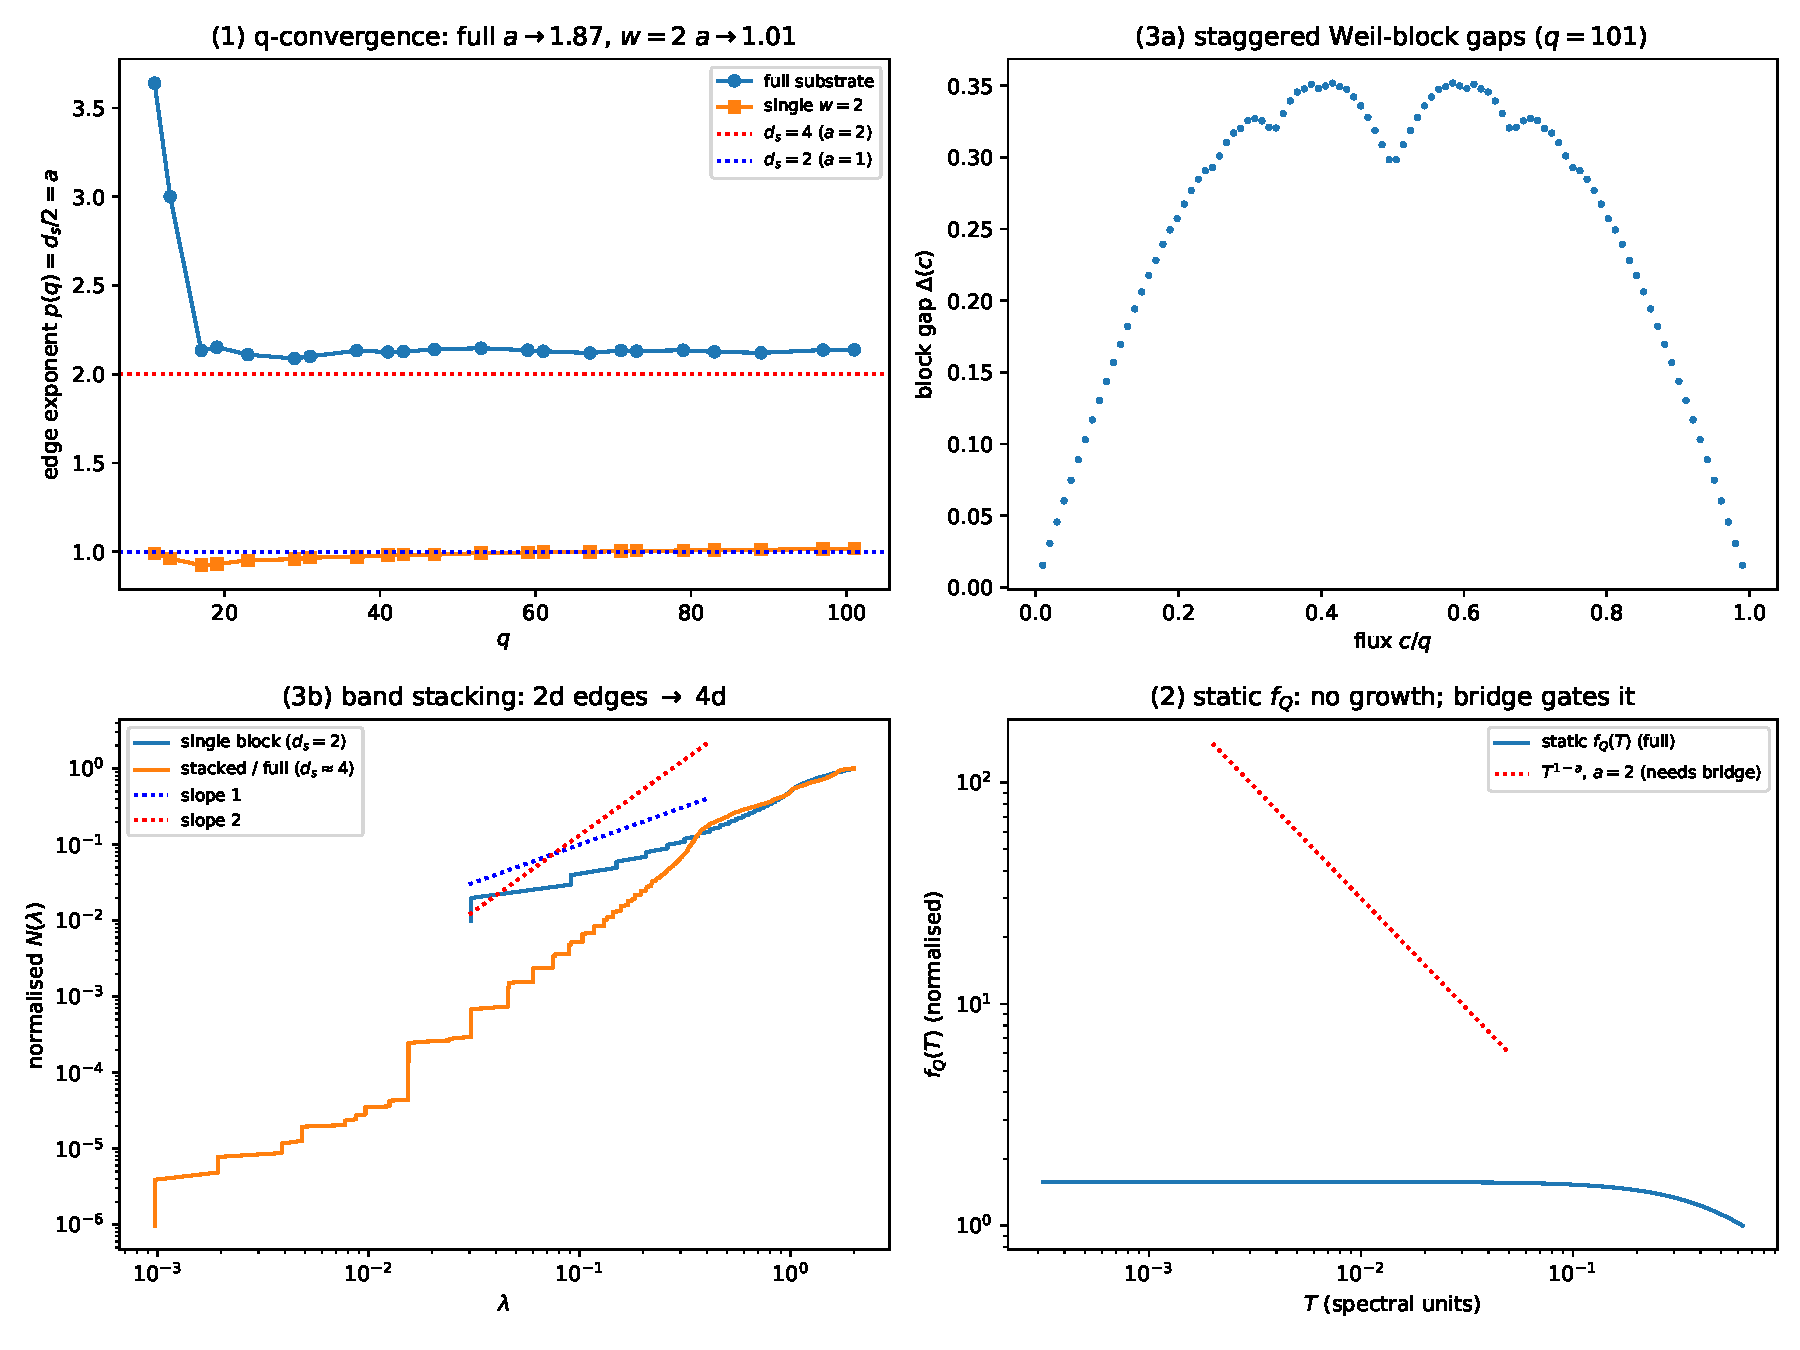
\includegraphics[width=0.99\textwidth]{qfi_refine}
\caption{Refinements from the exact block decomposition~\eqref{eq:decomp}.
Top left: $q$-convergence of the edge exponent $p(q)=d_s/2=a$, extrapolating to $a\to 2$ for the full substrate and
$a\to 1$ for the single $w=2$ block.
Top right: the staggered Weil-block gaps $\Delta(c)$ against flux $c/q$.
Bottom left: band stacking, the single-block counting function (slope $1$, $d_s=2$) against the full one
(slope $2$, $d_s=4$).
Bottom right: the static-spectrum $\fQ(T)$ is flat-to-decreasing by the sum rule, so the observed growth is not
produced by the static substrate and requires the thermal closure $\DPi(T)\sim T$.}
\label{fig:refine}
\end{figure}

\section{Thermal closure from the heat-kernel flow}
\label{sec:thermal}

The growth of $\fQ(T)$ requires the scaling form $\chi''(\omega,T)=T^{-a}\Phi(\omega/T)$, equivalently a thermal
closure of the gap, $\DPi(T)\sim T$.
This is not an extra assumption: it follows from the framework's own identification of the heat-kernel scale with
inverse temperature.

The local spectral energy density of the framework is $u(x;t)=-\partial_t\log K(x,x;t)$, the analogue of
$E=-\partial_\beta\log Z$, so the diffusion scale $t$ plays the role of $\beta=1/T$~\cite{Beau2026Thermodynamics}.
The linearised relaxation dynamics of the substrate is the heat-kernel flow $e^{-\Lap t}$.
With the trace return $P(t)=\frac1N\,\mathrm{Tr}\,e^{-\Lap t}=\frac1N\sum_n e^{-\lambda_n t}$, the effective gap at
temperature $T$ is
\begin{equation}
\DPi(T)\;\equiv\;u(1/T)\;=\;-\partial_t\log P(t)\big|_{t=1/T}\;=\;
\frac{\sum_n\lambda_n e^{-\lambda_n/T}}{\sum_n e^{-\lambda_n/T}}.
\label{eq:ut}
\end{equation}
For an edge density of states $\rho(\lambda)\sim\lambda^{d_s/2-1}$ one has $P(t)\sim t^{-d_s/2}$, hence
\begin{equation}
\DPi(T)=\frac{d_s}{2}\,T,
\label{eq:planckian}
\end{equation}
linear in temperature with slope $d_s/2$.
This is the Planckian closure, derived rather than assumed.

Exact assembly of the full spectrum confirms equation~\eqref{eq:planckian}: the product $u(t)\,t$ plateaus at
$d_s/2$, with median values $2.07$, $2.04$, $2.03$ at $q=61,101,151$, converging to $2$, that is $d_s=4$.
Figure~\ref{fig:thermal} shows the plateau and the linear closure $\DPi(T)\sim 2T$.
Combined with the power-law density of states of Sections~\ref{sec:full} and~\ref{sec:stacking}, scale invariance
then fixes $\chi''(\omega,T)=T^{-a}\Phi(\omega/T)$ with $a=d_s/2$, and equation~\eqref{eq:scaling} gives
$\fQ(T)\sim T^{1-a}=T^{-1}$ for the full substrate.
The chain from the substrate to the scale-free QFI growth is thereby closed at the level of the linear
(heat-kernel) dynamics.
\emph{Status: derived (the heat-kernel identification of $t$ with $1/T$ and the linear flow); the Born--Infeld
nonlinearity of the full relaxation dynamics is a correction near saturation, and is the natural candidate to
soften the exponent from $\alpha_{\mathrm{th}}=1$ towards $\alpha_{\mathrm{exp}}\approx 0.7$.}

\begin{figure}[t]
\centering
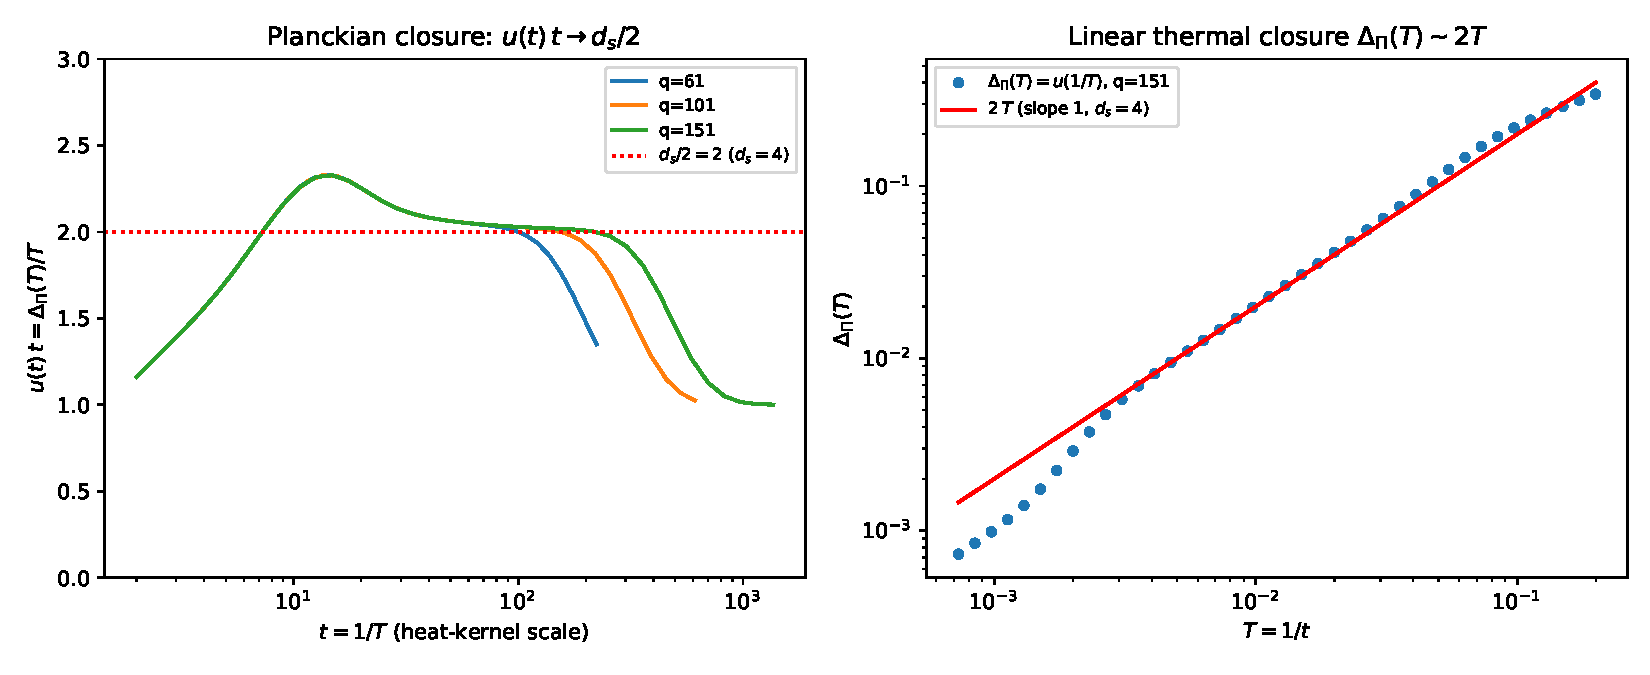
\includegraphics[width=0.92\textwidth]{thermal_closure}
\caption{Thermal closure from the heat-kernel flow.
Left: $u(t)\,t=\DPi(T)/T$ plateaus at $d_s/2$ across $q$, converging to $2$ ($d_s=4$).
Right: the effective gap $\DPi(T)=u(1/T)$ against $T$, following the linear law $\DPi(T)\sim 2T$.}
\label{fig:thermal}
\end{figure}

\section{Discussion}
\label{sec:discussion}

\subsection{Comparison with the experiment}

\begin{remark}[Material bridge]
The present note does not derive a microscopic Kondo-destruction model of $\mathrm{Ce}_3\mathrm{Pd}_{20}\mathrm{Si}_6$.
It tests a more limited question: whether the infrared type seen by the QFI witness, namely scale-free multipartite
entanglement rather than saturation or marginal logarithmic growth, is compatible with the projective spectral data
of the framework.
The material-specific spin dynamics, form factors, and saturation level enter as bridge data; the structural output
is the regime and its spectral origin, while the observed exponent is a separate material-level value.
\end{remark}

The experiment reports a scale-free increase of the QFI density by a factor of about forty between $10\,$K and
$60\,$mK~\cite{Mazza2026}.
Read as a power law over that range this corresponds to an exponent $\alpha_{\mathrm{exp}}\approx 0.7$, that is
$a_{\mathrm{exp}}\approx 1.7$.
The full-substrate value $a\approx 2$ gives $\alpha_{\mathrm{th}}\approx 1$.
The framework therefore predicts the correct regime, a power law rather than saturation or marginal growth, and
the correct order of magnitude, while overestimating the exponent.
\emph{Status: conditional.}

It is worth separating the two halves of this comparison.
The regime, a power law with $\alpha=1$ rather than saturation or marginal growth, follows from the edge spectral
dimension $d_s=4$ and the thermal closure of Section~\ref{sec:thermal} alone, with the neutral, mode-uniform weight
$w(\lambda)\equiv 1$; the flat weight is the unbiased choice, not a witness tuned to the data, so the regime is
obtained without any free adjustment.
The value $\alpha\approx 0.7$ is a logically separate question, controlled by the Born--Infeld softening of
Section~\ref{sec:binl} and not by the weight.
The staggered $d$-wave witness discussed next is therefore not a candidate that ``should" reproduce the value and
fails; it is a test establishing that the matrix-element weight is the wrong lever for the value (it moves $a$ the
wrong way), which is precisely why the lever is the Born--Infeld nonlinearity.
The required honesty therefore bears on the value, not on the regime: ``right order but steeper" is exact, and the
regime itself holds without tuning.

The overestimate is not removed by the matrix-element weight of the physically grounded witness.
The staggered $Q=(\pi,\pi)$ operator of the superconductivity construction~\cite{Beau2026g}, with its $d$-wave
$B_{1g}$ form factor $(\cos k_x-\cos k_y)$, has a node at the band bottom, so it suppresses the lowest modes and
\emph{raises} the effective exponent (on the abelian torus sector, from $a\approx 1$ to $a_{\mathrm{eff}}\approx 3$),
steepening the predicted growth rather than flattening it.
Lowering $a$ towards $\alpha_{\mathrm{exp}}$ would instead require an infrared-enhancing coupling, which the
grounded witness is not.

\subsection{Relation to the effective entanglement observable}

The effective entanglement observable of the framework, $E_{\mathrm{eff}}(C)=\DPi(C)\,(1-C^\nu)$~\cite{Cosmochrony},
is proportional to $\DPi$ and therefore \emph{vanishes} as the gap closes, whereas the QFI density \emph{diverges}
as the gap closes when $a>1$.
The two are distinct, complementary witnesses: $E_{\mathrm{eff}}$ counts entanglement generated during a discrete
reorganisation event, proportional to the gap, while the QFI density counts the multipartite correlation depth of
the steady state, which grows as the gap closes.
The QFI is thus a genuinely new spectral witness in the framework, not a re-expression of $E_{\mathrm{eff}}$ or of
the projection-entropy bound of the Bell paper~\cite{Beau2026b}.
Its natural home is the entanglement sub-programme~\cite{Beau2026entnote, Beau2026ent1}.
\emph{Status: structural.}

\subsection{Born--Infeld nonlinearity}
\label{sec:binl}

The derived exponent $\alpha_{\mathrm{th}}=1$ uses the effective linear heat-kernel response.
The full bounded-response correction is Born--Infeld in character~\cite{Cosmochrony}: near saturation the admissible
response rate is capped, so high-stress regions contribute less efficiently than they would in the linear flow,
\begin{equation}
\dot\phi_i = -\sqrt{\max(0,1-S_i)}\,(\Lap\phi)_i,\qquad
S_i=\frac{1}{c_{\mathrm{BI}}^2}\sum_{j\sim i}(\phi_i-\phi_j)^2,
\label{eq:biflow}
\end{equation}
so that high-stress nodes freeze while low-gradient modes relax linearly.
This correction should be read as an effective response correction, not as a fundamental substrate dynamics.
Simulating this flow on the substrate and reading the effective gap $u(t)=-\partial_t\log C(t)$ from the return
$C(t)=\langle\phi(0),\phi(t)\rangle/\lVert\phi(0)\rVert^2$ shows that the nonlinearity bends the effective exponent
\emph{downward} from the linear value.
On a fixed temperature window the crossing $\alpha_{\mathrm{eff}}=0.7$ occurs at a mean substrate saturation
$\langle S\rangle\approx 0.21$, stable across four system sizes: $\langle S\rangle_c=0.201,\,0.205,\,0.219,\,0.211$
for $q=13,17,19,23$, with no systematic drift (the spread is statistical, of order $\pm 0.01$).
The bent exponent runs weakly with temperature rather than being a pure power law, the saturation required for
$\alpha_{\mathrm{eff}}=0.7$ decreasing from $0.23$ to $0.16$ across the accessible window.
Figure~\ref{fig:binl} shows the effective exponent against saturation and the size stability of the crossing.
\emph{Status: numerical. The direction (the nonlinearity lowers the exponent) and the size-stable crossing are
robust; the running of the exponent and the saturation level of the physical system are not pinned, and the
asymptotic value is not derived.}

\begin{figure}[t]
\centering
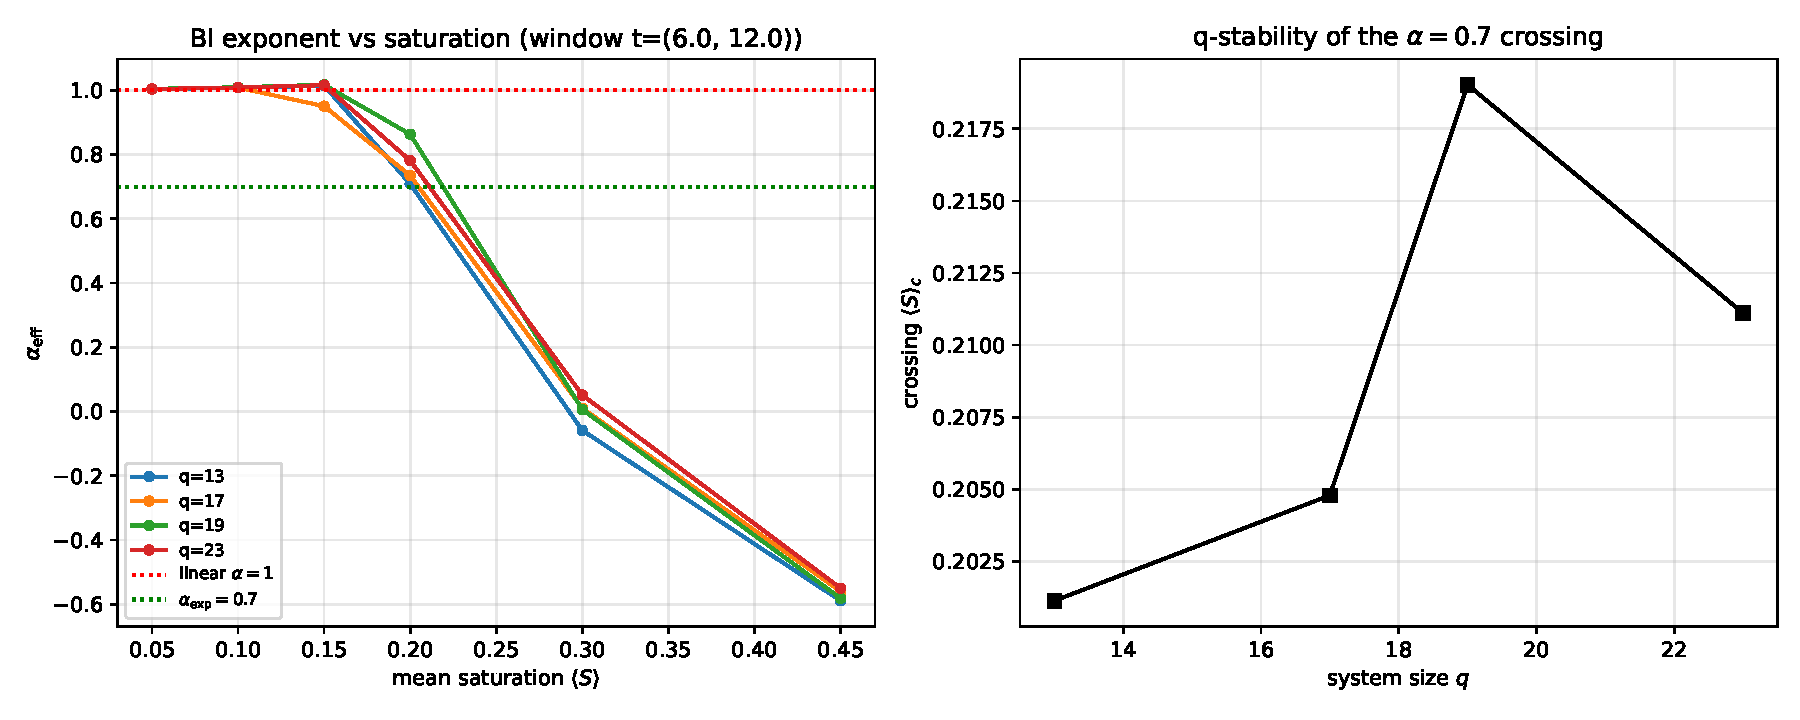
\includegraphics[width=0.99\textwidth]{bi_extend}
\caption{Born--Infeld nonlinearity from equation~\eqref{eq:biflow}.
Left: the effective exponent $\alpha_{\mathrm{eff}}$ against mean saturation $\langle S\rangle$, read on the fixed
window $t\in[6,12]$; the curves for $q=13,17,19,23$ overlap and the $\alpha_{\mathrm{eff}}=0.7$ crossing sits at
$\langle S\rangle\approx 0.21$.
Right: the crossing $\langle S\rangle_c$ against system size $q$, stable to within $\pm 0.01$ with no systematic
drift.}
\label{fig:binl}
\end{figure}

\subsection{Open directions}

The thermal closure that was the decisive gate is now derived in Section~\ref{sec:thermal}, so the open items are
reduced and reframed.
First, the matrix-element weight $w(\lambda)$ of the witness operator is anchored rather than free: the physically
grounded witness is the staggered $Q=(\pi,\pi)$ operator of the superconductivity construction~\cite{Beau2026g},
with $d$-wave $B_{1g}$ form factor $(\cos k_x-\cos k_y)$, realised basis-free as $O_d=A_X-A_Y$.
Its form factor has a node at the band bottom, so it suppresses the lowest modes and \emph{raises} the effective
exponent rather than lowering it; it therefore does not close the gap with $\alpha_{\mathrm{exp}}$.
Since $O_d$ annihilates the constant ground mode, $A_X\mathbf{1}=A_Y\mathbf{1}=2\,\mathbf{1}$, its weight is a
finite-temperature quantity tied to the thermal flow of Section~\ref{sec:thermal}.
Second, the Born--Infeld nonlinearity of the full relaxation dynamics, which corrects the linear heat-kernel flow
near saturation.
Section~\ref{sec:binl} shows numerically that this correction softens the derived exponent $\alpha_{\mathrm{th}}=1$
towards the observed $\alpha_{\mathrm{exp}}\approx 0.7$, with a crossing stable across four sizes
($q=13,17,19,23$) at $\langle S\rangle\approx 0.21$.
What remains open is the asymptotic value of the running exponent and the saturation level of the physical system,
hence the step from a derived regime and a confirmed mechanism to a derived value.
\emph{Status: the thermal closure is derived; the Born--Infeld softening is numerically confirmed and size-stable,
with its asymptotic value open.}

\section{Conclusion}
\label{sec:conclusion}

We have reduced the quantum Fisher information density to the projective spectral data of Cosmochrony and shown
that scale-free growth is equivalent to a closing gap together with an edge spectral dimension $d_s>2$.
Exact diagonalisation then separates two cases.
The single winding sector $w=2$, which is a critical almost-Mathieu operator, is marginal ($d_s=2$, $a=1$).
The full nilpotent substrate, of homogeneous dimension $D=4$, is power-law ($d_s\approx 4$, $a\approx 2$), and
reproduces the regime and order of magnitude of the measured QFI growth.
The thermal closure $\DPi(T)=\tfrac{d_s}{2}T$ required for that growth is derived from the framework's heat-kernel
identification of the diffusion scale with inverse temperature, so the chain from the substrate to
$\fQ(T)\sim T^{-1}$ closes at the level of the linear relaxation dynamics, the Born--Infeld nonlinearity remaining
the single residual input.
The scale-free entanglement signature of the strange metal is, in this framework, a property of the full substrate
rather than of any isolated composite, in keeping with the collective, multipartite character of the measured
state.

\newpage
\bibliographystyle{plain}
\bibliography{quantum_fisher_witness}

\end{document}
